\documentclass[11pt]{article}
\usepackage[utf8]{inputenc}
\usepackage{geometry}
\geometry{a4paper, portrait, margin=3cm}
\usepackage{graphicx}
\usepackage{amsmath, amssymb}
\usepackage{lineno}
\usepackage{cite}

\usepackage{float} % set figure location

\usepackage{helvet}
\renewcommand{\familydefault}{\sfdefault}
\usepackage{amsmath}
\usepackage{setspace}
\usepackage{indentfirst}
\usepackage{siunitx}
\usepackage{parskip}
\usepackage[labelfont=bf]{caption}
\usepackage[authoryear]{natbib}
\usepackage[T1]{fontenc}
\usepackage{multirow}
\usepackage{multicol}
\usepackage{rotating}



\linespread{1.5}

\begin{document}
 
\begin{titlepage}
		
\begin{center}
			
\begin{figure}[t]
\centering

\includegraphics[width = \textwidth]{../Code/Materials/logo.jpg}
\end{figure}

		\vspace{1cm}
\Huge
\textbf{The comparison of fitness of mechanistic vs. phenomenological microbial population growth models based on an empirical dataset }\\
		
		\vspace{3cm}
		\Large
		
	
		\textbf{MSc Computational Methods in Ecology and Evolution}\\
		\textbf{Department of life Science}\\
		\textbf{Imperial College London}\\
		\vspace*{1cm}
 		\textbf{Yuan Zhang}\\   
		\textbf{yuan.zhang119@imperial.ac.uk}\\
		\vspace*{2cm}	
		\textbf{Word count: 3055}\\

		
		\end{center}

	\end{titlepage}
	
	\clearpage
	\tableofcontents
	
	
	\linenumbers %show line numbers
	\doublespacing



\newpage

\section*{Abstract}
There is an essential function of the fluctuations in single population abundance for the ecosystem dynamic and functional characteristics. In this experiment, focusing on 4 models (Logistic model, Gompertz model, Baranyi model, as well as the Buchanan model), fit probability and the probability of becoming the best fit model were tested based on 275 data sets. As a result, it was found that the Logistic model has a large probability of fit but 2 phenomenological models (Gompertz model, Baranyi model) have better fitness. The Buchanan model shows very low levels in both the probability of fit and the probability of best fit. Comparisons between the models are discussed. Moreover, temperature as an environmental factor has also been studied and discussed. Finally, based on this experiment and other researches, ideas and suggestions for future modeling were proposed.  


\section{Introduction}  
As an indispensable part of population research, microbial growth has been extensively studied. There is an essential function of the fluctuations in single population abundance for the ecosystem dynamic and functional characteristics. Additionally, population growth was described as a reliable index to reflect biological responses \citep{R7}. Some issues could be investigated and predicted by focusing on microbial growth. Notably, in terms of risks of food poisoning, caused by food spoilage, pathogen growth will consequently raise a common issue of public health risk \citep{R6}. Besides, tumor growth pasterns also play a crucial role in the ongoing battle against cancer \citep{R1, R2}. A miscellany of new strategies, experimental techniques and theoretical approaches can be integrated into the struggle against the cancer. However, to explain and interpret the experimental discoveries, researchers usually make the best use of recourse to mathematical models based on previous cancer researches in many aspects and fields. Therefore, scientists has become conscious  of the possibilities of mathematical models, realizing that the existing medical techniques and experimental methods can not be able to tell the differences between a variety of possible mechanisms underlying key aspects of tumour evolution\citep{R2}.

The population is usually growing in an exponential way at the beginning, based on the low abundance and unlimited resources on the basis of the Malthusian principle \citep{R9}. Before the population grows fast, there exists a time lag. As time goes by, the population is growing more and more slowly and finally at a relatively stable balanced point because of limitations in several aspects. It is essential to pay much attention to microbial growth rates. Particularly, the latter one in batch culture usually has a specific series of phases. The first one is named as the lag phase, in the course of which a series of transcriptional machinery can be stimulated, such as the genes referring to the nutrient uptake and metabolic change for the preparations for bacteria growth. The second phase is called the exponential growth phase, in which the number of bacteria at a steady speed and the amount will double with every generation. The growing speed will not slow down until it reaches the carrying capacity of the media. Then it will step into a stable status for the population, entering the followed phase called the stationary phase.  

In previous studies, one of the measurements to determine the microbial growth rate is widely used \citep{R6, R10}. As Figure1 presents, explicitly, it plots the cell number or density against time on a semi-log graph and to fit a straight line through the exponential growth phase – the slope of the line shows the highest growth rate. It is also practical to develop the models to depict the entire sigmoidal bacterial growth curve. Bacterial growth usually reflects a phase where the specific growth rate begins at the point of zero. Next, it will speed up to a high-level value within one particular period of time, leading to a lag time($t_{lag}$). Moreover, the growth curve will cover a final phase where the rate comes down and eventually to zero; that is, it will reach an asymptote (Nmax) \citep{R4}. In Figure 1, the growth curve can be defined as the logarithm of the number of organisms plotted against time, and the results vary to the changes of growth rates in a sigmoidal curve, having a lag phase merely behind t=0 followed by an exponential phase and next by a stationary phase. In addition to the lag period and the asymptotic value, there is some other valuable parameter of the growth curve, meaning the maximum specific growth rate($r_{max}$). The slope of the line determines $r_{max}$ on the condition that the organisms have an exponential growth since the logarithm of the number. 

\begin{figure}
\centering 
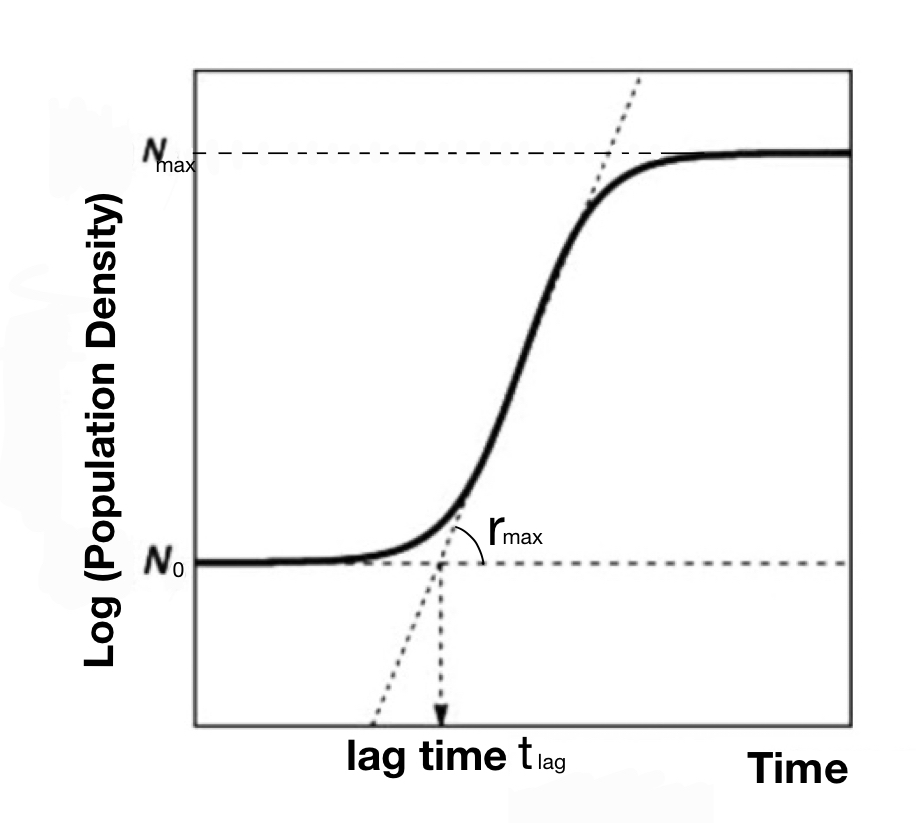
\includegraphics[width = 0.6\textwidth]{../Code/Materials/figure1.jpg}
      \caption{ A growth curve of semi-log density against time (this is a modified version from Zwietering et al. (1990))}
\end{figure}

Mathematical models have been applied and complicated with various parameters in bacterial growth studies, while different models have different results to some degree. Most models can be classified into two types: mechanistic and phenomenological ones and applications \citep{R6}. Given that a mechanistic model provides a tentative kinetic explanation of growth, it can be extensively applied in a large class of cases \citep{R12}. Particularly, a classical mechanistic model is called the logistic (Verhulst) equation, which has various modifications in former researches \citep{R12, R11, R13}.  Buchanan model \citep{R16} is also mechanistic as it could be considered as a 'three-phase logistic mode'. Different from the mechanistic ones, phenomenological models often are not derived from first principles, describing the empirical connection of phenomena. Several phenomenological growing models can be referred from literature, including the modified Gompertz model \citep{R10} and Baranyi model \citep{R14, R15}. To explain the curve and reduce the measured samples to a limited number of valuable parameters, the adequate models are necessary for the researchers. 

This project aims to compare the fitness of 4 mathematical models (two mechanistic model: Logistic equation and the Buchanan model; two phenomenological models: the Gompertz model and the Baranyi model ) based on a large dataset of microbial population growth cases. Moreover, this paper will also discuss if there is an existence of the interaction between temperature and model fitting, given that the temperature factor was not written in any model. The hypotheses are:
(1) Mechanistic models fit better than phenomenological ones in a large number of cases
(2) Gompertz model fit better than the Baranyi model  
(3) Temperature does not affect which population growth rate model fits best

		
\section{Methods}
\subsection{Data and preparation before the modelling }
The original dataset called $LogisticGrowthData.csv$ was used in this project. Collected from different studies, it contains measurements of change in biomass or number of cells of microbes over time. These data were collected through lab experiments across the world. The field names were defined in a file called $LogisticGrowthMetaData.csv$, also in the data directory. The two main fields of interest are $PopBio (abundance)$ and $Time$. 

Data were modified with unique single IDs and unsuitable and low-quality data were deleted. Single population growth rate curves can be identified as unique temperature-species-medium-citation-replicate combinations (concatenate them to get a new string variable that identifies unique growth curves).  In addition, NA, negative, duplicated data were filtered and removed. Besides, datasets with less than 5 data points were also filtered out and removed where 5 is the minimum number of data points needed to fit the models. After the modification, the dataset composed by 4225 observations, 45 species with 275 unique IDs and temperature. 

\subsection{Models}
\subsubsection{Mechanistic Model}
 A classical mechanistic model, is the logistic equation:
 \begin{equation}
N_t = \frac{N_0 * N_{max} * e^{r_{max} * t}} {N_{max} + N_0 * (e^{r_{max} * t} - 1)}
\end{equation}

Here $N_t$  is population size at time $t$, $N_0$ is initial population size, $r$ is maximum growth rate (AKA $r_{max}$), and $N_{max}$ is carrying capacity.

\paragraph{} The Buchanan model, considered as a 'three-phase logistic mode', is relatively simple:
\begin{equation}
    N_t = \begin{cases}
          N_0 & \text{if } t\leq t_{lag}\\
          N_{max} + r_{max} * (t - t_{lag})  & \text{if } t_{lag} < t < t_{max}\\
          N_{max} & \text{if } t\geq t_{max}
          \end{cases} \label{eq:Buchanan Model} \tag{2}
\end{equation}

\subsubsection{Phenomenological Model}
One of popular phenomenological model is called modified Gompertz model\citep{R10}: 
\begin{equation}
N_t = A*e^{-e^{\frac{r_{max}*e*(t_{lag} - t)}{A} + 1}} \tag{3}
\end{equation}

where $r_max$ maximum growth rate, the tangent to the inflection point.  $t_lag$ is the x-axis intercept to this tangent (duration of the delay before the population starts growing exponentially) and $A$ is the asymptote ($A$=ln($N_{max}$/$N_0$)), $N_0$ is initial cell culture (Population) density, $N_{max}$ is maximum population density.

Another  phenomenological model, called as Baranyi model, introduces a new dimensionless parameter $h_0$ which represents the initial physiological state of the cells. The length of the lag phase is determined by the value of $h_0$ at inoculation and the post-inoculation environment. Thus the definition of lag is independent from the shape of the growth curve, and the effect of the previous environment is separated from the effects of the present environment. This allows modeling growth without a lag period following inoculation from media favorable to growth to new media also favorable to growth.   $r_max$ and $h_0$ can be related to obtain the lag time, $t_{lag}$. The  formulation given is:
\begin{equation}
N_t = N_0 + r_{max}*{A_t} - ln(1 + \frac{e^{r_{max}*{A_t}} -1}{e^{N_{max} - N_0}}) 
\label{eqn:Baranyi} \tag{4}
\end{equation}
where: 
\begin{equation}
A_t = t + (\frac{1}{r_{max}}) * ln(\frac{e^{-r_{max}*t} + h_0} {1 + h_0})
\label{eqn:Baranyi_A} \tag{4.2}
\end{equation}

\begin{equation}
t_{lag} = \frac{ln(1 + \frac{1}{h_0})} {r_{max}}
\label{eqn:Baranyi_t} \tag{4.3}
\end{equation}


\subsection{Model fitting and Visualization}
A R script was written to get the model fitting named $ Model\_fitting.R$. Before fitting models to the dataset, the starting value of the parameters were calculated. For added complication, note that the biomass are written in log to the base 10, which means that data transformed to log base 10. These could also be written in the natural log too. The $r_{max}$ was derived from linear model. Start $N_{max}$ value was calculated by maximum of Log10N, while Start $N_0$ value was calculated by minimum of Log10N. Then 4 models mentioned above were used to investigate the model fitting with a loop. In the meanwhile, AIC and BIC for each model were calculated and stored in a file named $statistic\_data.csv$ in the Data folder. Consequently, dataset of each ID was plotted to figure. Those figures were saved as $respectiveplots$ to the $Results$ folder. 


\subsection{Model selection criteria}
4  models were compared and evaluated by Akaike information criteria(AIC) \citep{R17} and Bayesian information criterion (BIC) criteria \citep{R18}. The best model is the model with most support with lowest AIC or BIC. The best fitted models were counted and calculated the percentage for all datasets using the R script $results\_plotting.R$. Finally,  the data after criteria were plotted and saved to the folder $Results$.

\subsection{Computing languages}
Bash 3.2 : A file $compile.sh$ written in bash was used to compile the report into pdf format with bibliography. Another file $run_miniproject.sh$ writtern in bash aimed to run all the files and get the final results and report.

R 3.6.1: It was applied to get the data prepartion, calculate the criteria value, as well as plot the results. Some helpful packages were used. $dplyr$ was used to manage tables, $ggplot2$ was used for plotting, and $minpack.lm$ was used to conduct non-linear models. 

It needs to be pointed that, to take the most efficient work, in this research Python was not used, but It is undeniable that python still has related similar functions.

\section{Results}
\subsection{Fitting percentage of 4 models}
The four models are compared with respect to the probability of fitting to 275 data sets. It can be clearly seen in Figure 2 that the mechanistic model (Logistic) has the highest match rate (98.5\%). Two phenomena models (Baranyi and Gompertz) are also very high, which have 76.7\% and 88.7\% respectively. However, the fitting percentage of the Buchanan model is exceptionally low, indicating that less than half of the data set can be adapted to this model (41.8\%). 
		\begin{figure}[h]
		\centering
		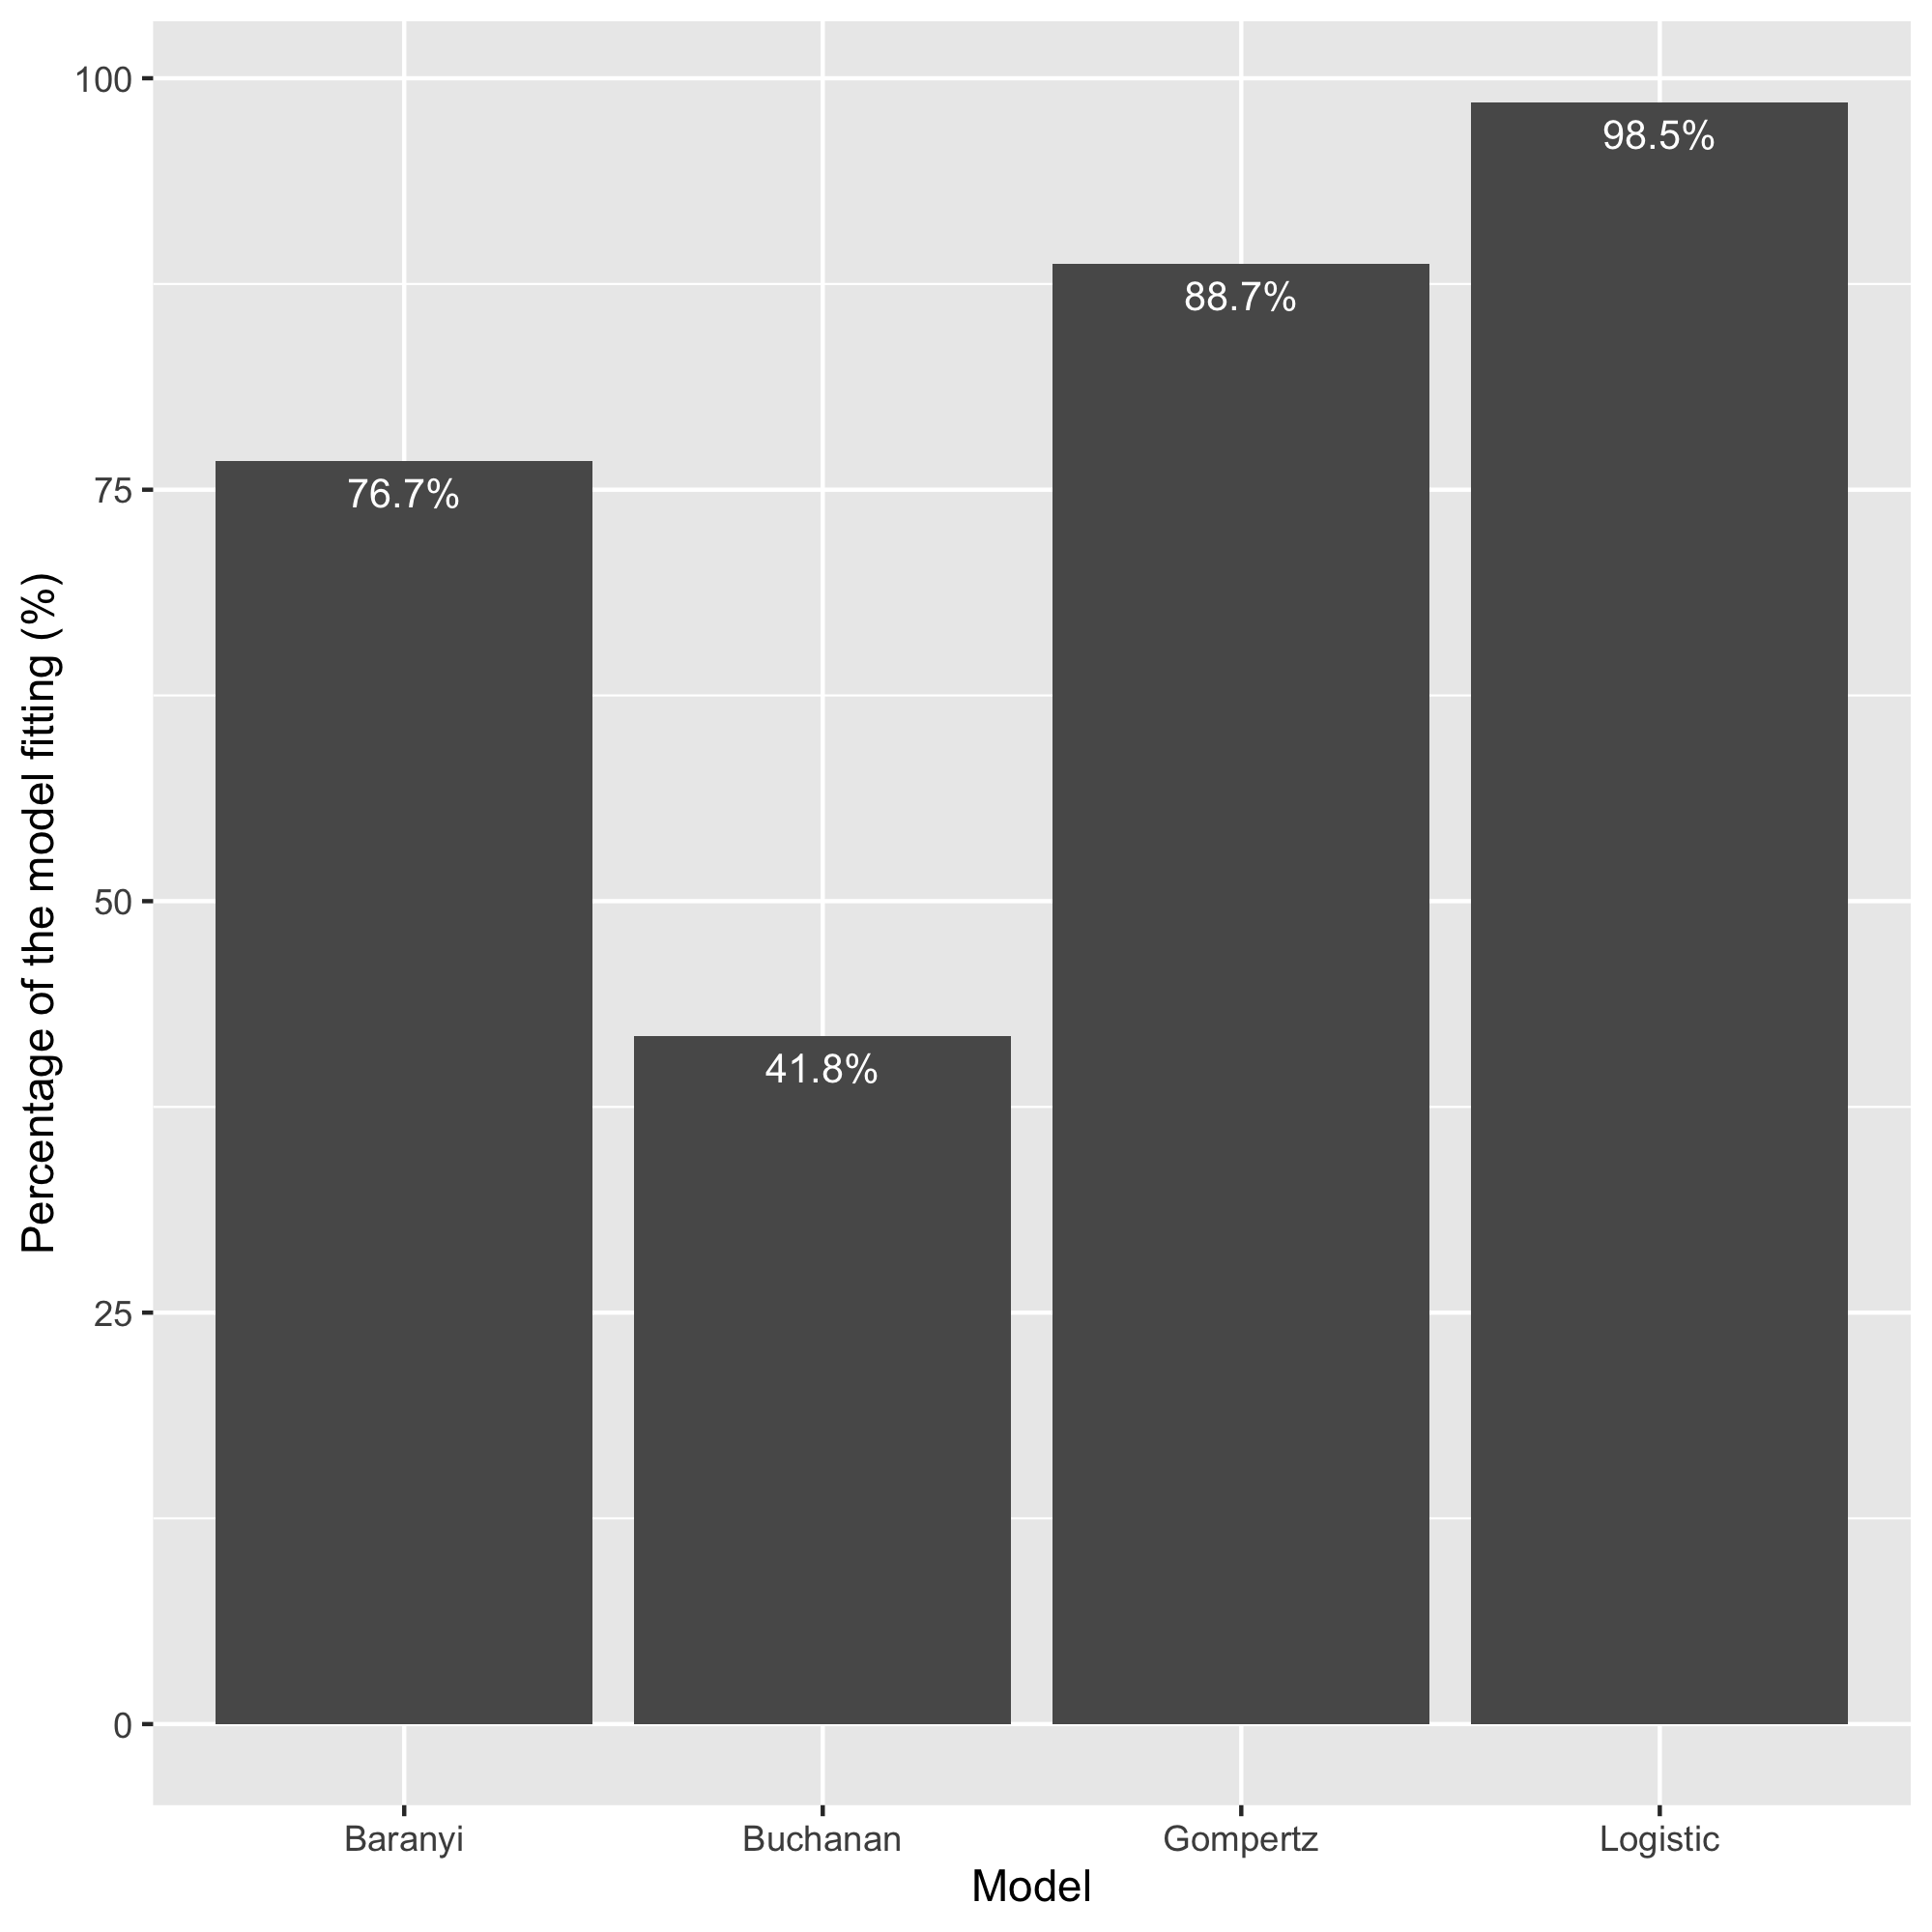
\includegraphics[width = 0.6\textwidth]{../Results/Fitting_percentage.png}
		      \caption{Figure 2. Percentage of model fitting}
	    \end{figure}
	    
\subsection{Best fitting model assessment}
Figure 3 shows the percentage of each model that was rated as the best fitting. It can be seen that both phenomena models (Baranyi and Gompertz) are higher than mechanical models (Logistic and Buchanan), of which the Gompertz model (37.5\% of AIC and 36.7\% of BIC) has the remarkably highest optimal rate. Whereas, the Buchanan model still gets a very deficient optimal percentage(10.2\% of AIC and 9.5\% of BIC). There are some differences between the fitness of the models and neither can consistently offer the best fit to almost every growth curve.
\begin{figure}[h]
\centering
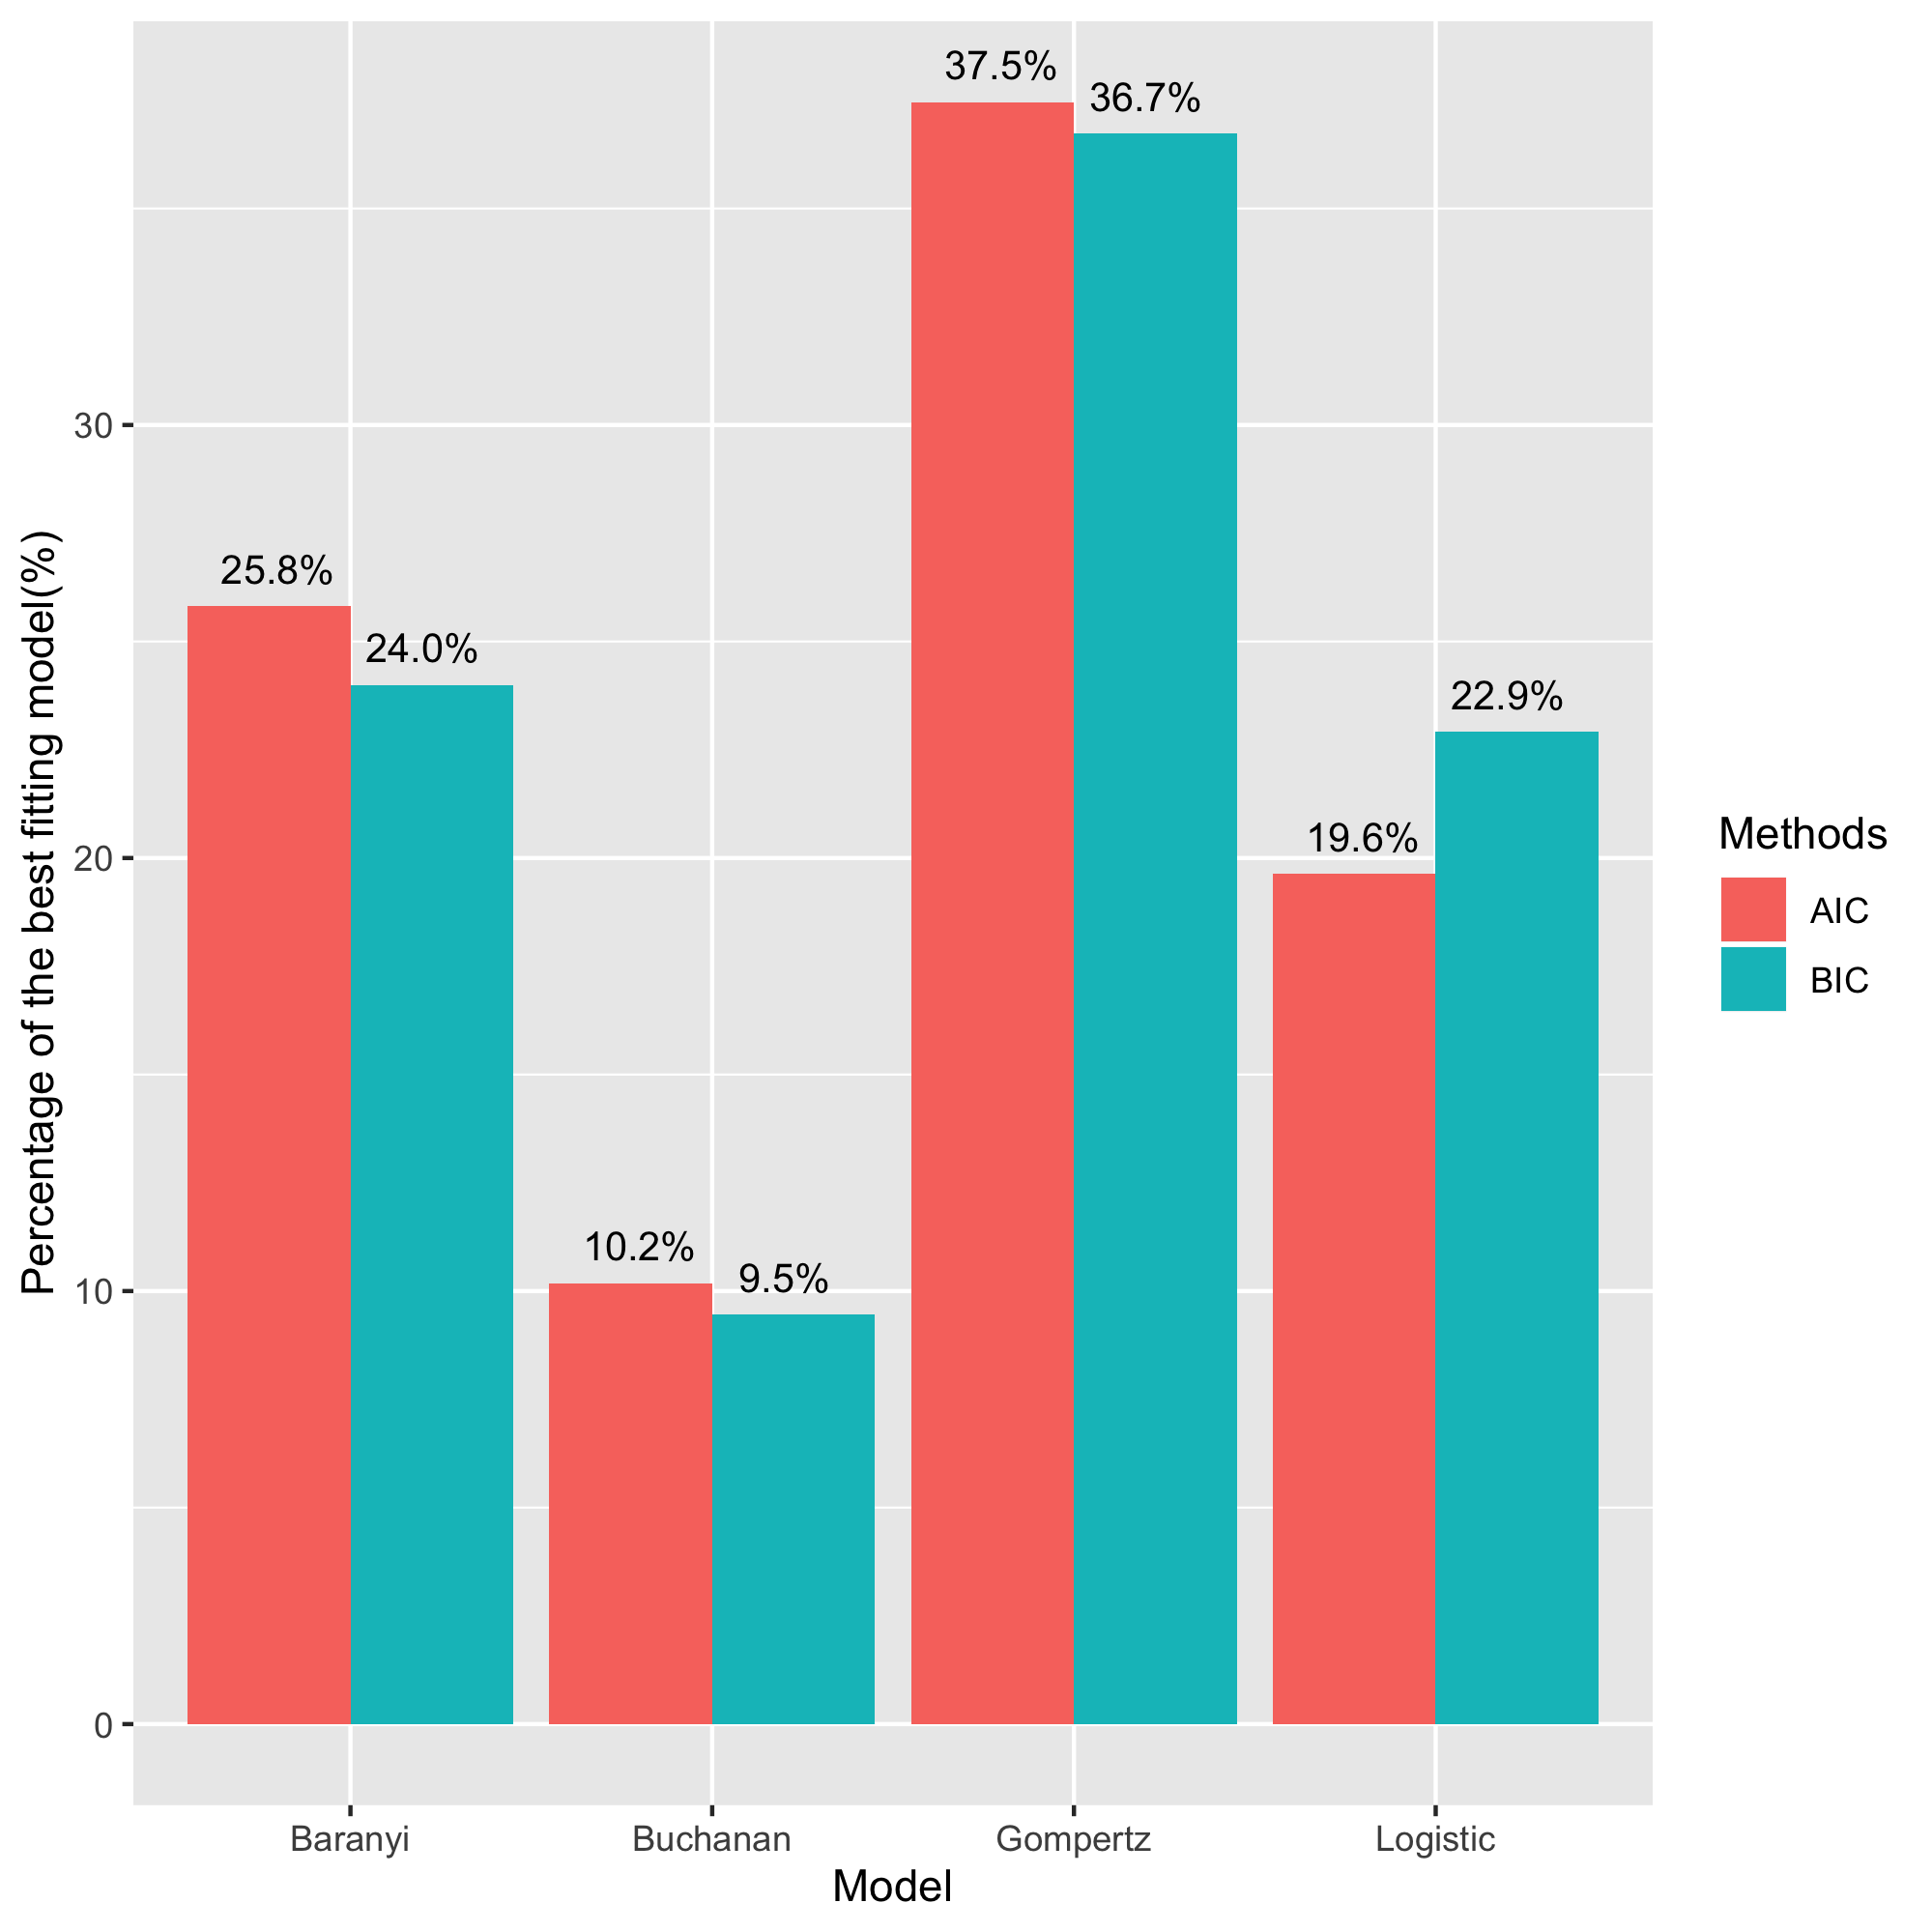
\includegraphics[width = 0.6\textwidth]{../Results/Bestfitting.png}
        \caption{Percentage of Best model fitting for each model}
	    \end{figure}


\subsection{Four model fittings on one species with different temperatures}
One species with different temperatures was selected randomly as an example to present the model fitting situations about this unique ID. The species is $Staphylococcus\,spp.$, whose database is focusing on the bacterial growth on the raw Chicken Breast \citep{R19}. This measurement has 6 types of temperature. Figure 4 shows that in this example, the result is that most models still have a relatively good fit at different temperatures. Therefore, specifically from this example, it is undeniable that the effect of temperature on the fitness of the model is basically non-existent. Moreover, it can be seen from Figure 4. b that when the temperature is 4 degrees Celsius, the data is relatively small, and the Buchanan model deviates significantly from the actual situation. It is worth mentioning that both in Figure 4.b and 4.c that there is a downward trend at the end period of each curve, but each model does not fit well and does not reflect the decreasing part. Furthermore, it also could be found that the Logistic model has an upturned part at the beginning of Figure 4.a, c, d, and e. Compared with other models, it does not fit well in the lag-time duration.
\begin{figure}[h]
\centering
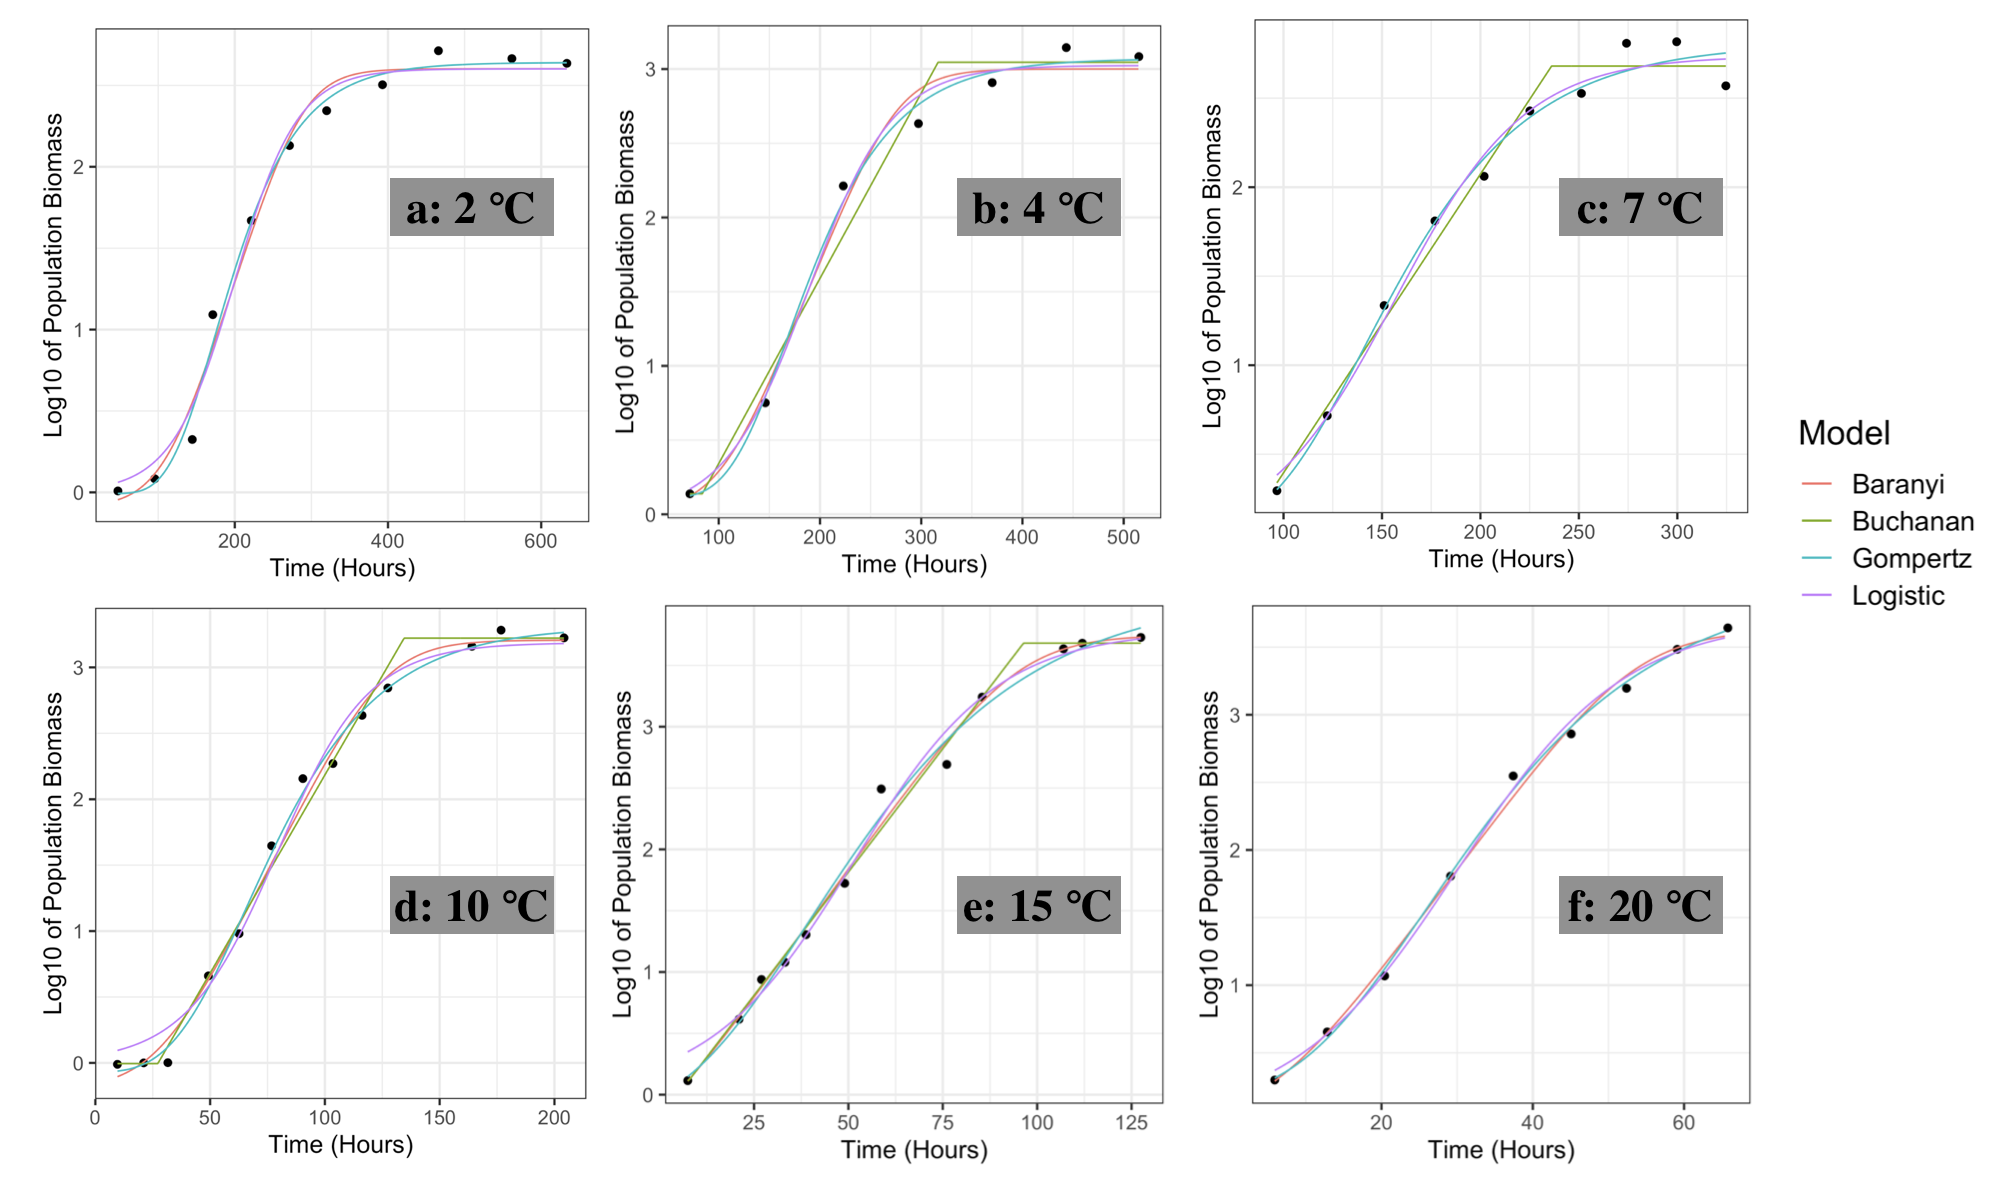
\includegraphics[width = \textwidth]{../Code/Materials/figure4.jpg}
       \caption{Four model fittings on one species ($Staphylococcus\,spp.$) with different temperatures }
	    \end{figure}


\section{Disscussion}
\subsection{Difference between phenomenological and mechanistic models}
The results in 3.1 show that when studying a large number of data sets, the Logistic model has the highest capacity for fitting probability. The reason is a mechanical model starting from the most basic growth theory. The results of 3.2 show that though the model is not as high as the mechanistic model, the Gompertz model still obtains the highest optimal adaptation rate, which is consistent with previous research that phenomenological models often perform better than mechanistic ones, for the former ones have less restrictive assumptions and uncertainty \citep{R21, R22, R23}. Thus, it will not tend to be applied on a large scale in modeling microbial growth and casualty. In addition, it is possible that although it totally lacks the mechanistic interpretation, the equation or the other empirical 4-parameter models, can be applied to fitting the experimental growth \citep{R20}. 

One of the standards of evaluating the phenomenological model is whether it is convenient to apply and accurate to offer a fit, without the basis of any basic principles or mechanistic considerations \citep{R6}. For instance, the parameters of the modified Gompertz equation have not been directly linked with microbial death kinetics when using the logarithmic number of cells \citep{R8}. 
The ‘three-phase logistic model‘, The Baranyi-Roberts Model presents easy mechanism and intuitive meanings, but shows low fitness and precision. Due to the two ’If‘ statements, the linear model could not be assessed that conveniently for the description and prediction of growth on dynamic conditions and then the transition between one phase and the next one will not tend to be sharp just like those in the other isothermal curves. 

\subsection{Comparison of 2 phenomenological models (Gompertz model and Baranyi model)}
The results also show that the Gompertz model is better than the Baranyi model, both in the possibility of fitting and best fitting rate. However, it is different from a study illustrating that taking the model generated data into consideration in a broad way, the results by Baranyi’s model can be more ideal than the modified Gompertz equation \citep{R8, R26}. Nevertheless, more literature argues the modified Gompertz equation was used primarily in modelling the asymmetrical sigmoidal shape of microbial growth curves \citep{R24, R4, R5}. The Gompertz model can offer a description of the growth curves with a short or long lag time or neither combined with the parameters’ adjustments \citep{R6}. However, the Baranyi model is better than the Gompertz one at higher growth rate samples \citep{R14}. 

There are some problems in the Baranyi model, one of which can be the meaning that the lag time defined has a close relationship with the maximum specific growth rate. In some favorable situation for the organism, someone can expect the growth not merely to be more vigorous, but also to begin earlier (manifested in a shorter lag time). Thus, it has discovered a negative relation between that lag time and maximum \citep{R25}. The Baranyi model can make a prediction that the extensions of almost every isothermal (semi-logarithmic) tangent of the growth curve at the inflection point must meet at one point. It is not merely inconsistent by some reported growth data in the article \citep{R8, R27}, but also proven not to be accurate by simulating realistic growth curves with the Gompertz as a model violating the rule. 
 
\subsection{Temperature factor}
Although on the basis of the frequent observation, there are not any reasons in the aspect of theories that the growth parameters are always rising and falling in unison, keeping pace with changes in the external condition. Therefore, to quantify the effects of the environmental factors on microbial growth needs, the growth parameter should be assessed, not merely considering the maximum specific growth rate. The results vary to the selected methods with determining the “lag time” often yield different values, showing that it is not an inadequate definition of growth parameters. The simultaneous effects of the factors, including T, pH, or aw, should not be multiplicative but be evaluated via experiments \citep{R6}. However, the result 3.3 shows that the temperature has little effect on fitness. The reason may be that several models can be performed at different temperatures. For instance, when the temperature dependence was assessed via a series of experiments, the Buchanan model will be applied to the generation of non-isothermal growth curve to some degree alike that in the biphasic survival curve \citep{R28}. Similarly, other models can make predictions about non-isothermal growth patterns according to isothermal data. Therefore, it is practical to select a relatively simple and convenient model \citep{R6}.

\subsection{Limitation and suggestions for future studies}
This article has many limitations. First of all, there are some data from other literature, and there are strange distributions, which may be due to simultaneous mortality during bacterial growth. Moreover, although AIC and BIC are good candidates for modelling, the criteria used are limited. Moreover, in this experiment, the difference between AIC and BIC has not been thoroughly explored. In the case of extensive data, it is difficult to show all the adapted p-values. Those limitations could be considered in future studies. Furthermore, some research directed that the future of predictive microbiology may be altered from combining a phenomenological and mechanistic basis to complicated systems \citep{R5}. 


\section{Conclusion}
In conclusion, the hypothesis that the mechanistic model is better than the phenomenon model is unilateral. It requires different analysis in different situations. In this experiment, a large number of data sets were researched and found that although the logical model has a high probability of being fit, the phenomenon model can better fit the data set and better fit the degree. In addition, the Gompertz model fits best in phenomenological models in a large number of cases. 

Moreover, although the temperature did not show a significant impact on model adaptation in the study of a single example, it is recommended to consider the influence of environmental factors in future experiments. Generally, all models are optimized to generate a mortality phase by timing the original growth term by a decay factor, and it will be logistic, exponential, stretched exponential or any algebraic term that begins at 1 and drops to 0. A typical instance can be the model built for complicated chemical reactions and biological processes following the competing mechanisms \citep{R30}. Although it is evident that the observed growth pattern can be influenced by almost every factor above and their interactions, the shape of the growth curve cannot cover adequate data to assess the physiological influences of the changes singularly \citep{R29}.


\bibliographystyle{agsm}
\bibliography{Miniproject}

\end{document}